
\begin{table*}
\centering
{\small
    \begin{tabular}{|l|l|c|c|c|c|c|c|c|}
    \hline
	\multirow{2}{*}{~}			& \multirow{2}{*}{Approach}		& \multirow{2}{*}{\parbox{2.2cm}{Sleep Interval (seconds)}}	
																						& \multicolumn{3}{c|}{Average Power (mW)}		& \multicolumn{3}{c|}{Recall} 													\\ \cline{4-9}
								&								&						& Steps		& Headbutts	& Transitions	& Steps					& Headbutts					& Transitions 				\\ \hline
	\multirow{14}{*}{\parbox{1.2cm}{Group 1 90\% idle}}	& \multicolumn{2}{l|}{Always Awake}						& \multicolumn{3}{c|}{323}				& \multirow{6}{*}{98\%}	& \multirow{6}{*}{100\%}	& \multirow{6}{*}{100\%}	\\ \cline{2-6}
								& \multirow{5}{*}{Batching}		& 2						& \multicolumn{3}{c|}{350}				&						&							&							\\ \cline{3-6}
								& 								& 5						& \multicolumn{3}{c|}{186}				&						&							&							\\ \cline{3-6}
								& 								& 10					& \multicolumn{3}{c|}{115}				&						&							&							\\ \cline{3-6}
								& 								& 20					& \multicolumn{3}{c|}{80.1}				&						&							&							\\ \cline{3-6}
								& 								& 30					& \multicolumn{3}{c|}{68.3}				&						&							&							\\ \cline{2-9}
								& \multirow{5}{*}{Duty Cycling}	& 2						& \multicolumn{3}{c|}{339}				& 94\%					& 57\%						& 97\%						\\ \cline{3-9}
								& 								& 5						& \multicolumn{3}{c|}{217}				& 82\%					& 14\%						& 47\%						\\ \cline{3-9}
								& 								& 10					& \multicolumn{3}{c|}{140}				& 63\%					& 29\%						& 28\%						\\ \cline{3-9}
								& 								& 20					& \multicolumn{3}{c|}{86.3}				& 48\%					& 14\%						& 32\%						\\ \cline{3-9}
								& 								& 30					& \multicolumn{3}{c|}{63.1}				& 31\%					& 7\%						& 12\%						\\ \cline{2-9}
								& \multicolumn{2}{l|}{Predifined Activity}				& \multicolumn{3}{c|}{48.3}				& \multirow{3}{*}{98\%}	& 36\%						& 87\%						\\ \cline{2-6}\cline{8-9}
								& \multicolumn{2}{l|}{Smartsensor}						& 48.3		& 60.3		& 18.6			& 						& \multirow{2}{*}{100\%}	& \multirow{2}{*}{100\%}	\\ \cline{2-6}
								& \multicolumn{2}{l|}{Oracle}							& 41.5		& 59.6		& 16.4			& 						& 							& 							\\ \hline \hline
								
	\multirow{14}{*}{\parbox{1.2cm}{Group 2 50\% idle}}	& \multicolumn{2}{l|}{Always Awake}						& \multicolumn{3}{c|}{323}				& \multirow{6}{*}{99\%}	& \multirow{6}{*}{100\%}	& \multirow{6}{*}{100\%}	\\ \cline{2-6}
								& \multirow{5}{*}{Batching}		& 2						& \multicolumn{3}{c|}{350}				&						&							&							\\ \cline{3-6}
								& 								& 5						& \multicolumn{3}{c|}{186}				&						&							&							\\ \cline{3-6}
								& 								& 10					& \multicolumn{3}{c|}{115}				&						&							&							\\ \cline{3-6}
								& 								& 20					& \multicolumn{3}{c|}{80.1}				&						&							&							\\ \cline{3-6}
								& 								& 30					& \multicolumn{3}{c|}{68.3}				&						&							&							\\ \cline{2-9}
								& \multirow{5}{*}{Duty Cycling}	& 2						& \multicolumn{3}{c|}{334}				& 92\%					& 74\%						& 90\%						\\ \cline{3-9}
								& 								& 5						& \multicolumn{3}{c|}{243}				& 79\%					& 31\%						& 53\%						\\ \cline{3-9}
								& 								& 10					& \multicolumn{3}{c|}{176}				& 65\%					& 20\%						& 36\%						\\ \cline{3-9}
								& 								& 20					& \multicolumn{3}{c|}{106}				& 33\%					& 5\%						& 10\%						\\ \cline{3-9}
								& 								& 30					& \multicolumn{3}{c|}{80}				& 25\%					& 11\%						& 12\%						\\ \cline{2-9}
								& \multicolumn{2}{l|}{Predifined Activity}				& \multicolumn{3}{c|}{188}				& \multirow{3}{*}{99\%}	& 13\%						& 73\%						\\ \cline{2-6}\cline{8-9}
								& \multicolumn{2}{l|}{Smartsensor}						& 188		& 65.1		& 43.3			& 						& \multirow{2}{*}{100\%}	& \multirow{2}{*}{100\%}	\\ \cline{2-6}
								& \multicolumn{2}{l|}{Oracle}							& 153		& 62.3		& 29.5			& 						& 							& 							\\ \hline \hline

	\multirow{14}{*}{\parbox{1.2cm}{Group 3 10\% idle}}	& \multicolumn{2}{l|}{Always Awake}						& \multicolumn{3}{c|}{323}				& \multirow{6}{*}{97\%}	& \multirow{6}{*}{100\%}	& \multirow{6}{*}{100\%}	\\ \cline{2-6}
								& \multirow{5}{*}{Batching}		& 2						& \multicolumn{3}{c|}{350}				&						&							&							\\ \cline{3-6}
								& 								& 5						& \multicolumn{3}{c|}{186}				&						&							&							\\ \cline{3-6}
								& 								& 10					& \multicolumn{3}{c|}{115}				&						&							&							\\ \cline{3-6}
								& 								& 20					& \multicolumn{3}{c|}{80.1}				&						&							&							\\ \cline{3-6}
								& 								& 30					& \multicolumn{3}{c|}{68.3}				&						&							&							\\ \cline{2-9}
								& \multirow{5}{*}{Duty Cycling}	& 2						& \multicolumn{3}{c|}{332}				& 89\%					& 47\%						& 89\%						\\ \cline{3-9}
								& 								& 5						& \multicolumn{3}{c|}{257}				& 76\%					& 28\%						& 26\%						\\ \cline{3-9}
								& 								& 10					& \multicolumn{3}{c|}{198}				& 64\%					& 27\%						& 25\%						\\ \cline{3-9}
								& 								& 20					& \multicolumn{3}{c|}{133}				& 42\%					& 19\%						& 19\%						\\ \cline{3-9}
								& 								& 30					& \multicolumn{3}{c|}{99.1}				& 30\%					& 9\%						& 14\%						\\ \cline{2-9}
								& \multicolumn{2}{l|}{Predifined Activity}				& \multicolumn{3}{c|}{321}				& \multirow{3}{*}{97\%}	& 95\%						& 86\%						\\ \cline{2-6}\cline{8-9}
								& \multicolumn{2}{l|}{Smartsensor}						& 321		& 65.7		& 51.7			& 						& \multirow{2}{*}{100\%}	& \multirow{2}{*}{100\%}	\\ \cline{2-6}
								& \multicolumn{2}{l|}{Oracle}							& 266		& 62.9		& 34.9			& 						& 							& 							\\ \hline
    \end{tabular}
}
	\caption{Event recall and average power for synthetic traces.}
	\label{table:summaryRecallPower}
\end{table*}


\section{Results}
\label{sec:results}

In this section we first present the result of experiments conducted
on synthetic traces collected with our robotic testbed.  We then
present results from experiments on a small number of traces collected
from human subjects. 

% Finally, we discuss how an onboard Smartsensor
%implementation would affect our findings.

\subsection{Synthetic Traces}

We answer the following questions:

\begin{enumerate}
\setlength{\itemsep}{-3pt}  

\item What are the benefits of Smartsensor over Duty Cycling and
  Batching?

\item How flexible is Predefined Activity?

\item How much additional benefit can be obtained from fully
  programmable wake-up conditions?

\item Are multiple different filters required, and how important it is
  to let the application configure the filter parameters and
  thresholds?

\end{enumerate}

\subsubsection{Smartsensor vs. Duty Cycling and Batching}

Table~\ref{table:summaryRecallPower} presents the results of replaying
the traces collected from the robot for the sensing approaches
described in the previous section.  For each application, the table
presents average power consumption and activity recall.  Results are
averages across runs of the same group.  We use the results for the
Always Awake approach (which achieves close to perfect recall) as a
base line for comparison.  All sensing approaches achieved similar
average precision (Headbutts: 89\%, Transitions: 91\%, Walking:
93\%), and we therefore do not include these numbers in the table.

As expected, Duty Cycling performs poorly.  Short sleep intervals
actually result in an increase in power consumption due to frequent
transitioning between awake and asleep states.  Longer sleep interval
are more effective at saving energy, but they do so by sacrificing
recall.  For example, a sleep interval of 10 seconds reduces the
Headbutts and Transitions recall bellow 30\%.

Batching matches the recall of Always Awake, but requires long
batching intervals to achieve large energy savings.  Therefore, this
approach is not be appropriate for applications with timeliness
constrains.  For example, the user of a gesture recognition
application~\cite{liu2009uwave,schlomer2008gesture} would not be
satisfied if the application detects the performed gesture after a
delay of more than a couple of seconds.  We anticipate that in
practice realistic batching intervals are in the order of a few
seconds.  We therefore conclude, that batching will result in
significant energy waste for applications interested in low frequency
events (e.g., gesture recognition, fall detection).

Smartsensor matches the recall of Always Awake while achieving large
reductions in average power in all scenarios other than step detection
in Group 3, where walking represents 63\% of the trace and the device
experiences little sleep.  Smartsensor performed best when the event
of interest occurs infrequently, reductions power consumption by up to
94\%.  

\subsubsection{Smartsensor vs Predefined Activity}

Predefined Activity performs very well for step detection (as
expected), but results in either poor recall or low energy savings for
the other two applications.  We conclude that hardware support for
predefined activity detection may work well for specific use cases,
but lacks the generality to support a broad set of applications.


\subsubsection{Smartsensor vs. Oracle}

By comparing the performance of the Smartsensor approach to Oracle we
observe that for most usage scenarios, the Smartsensor approach
achieves over 95\% of the available power
savings\footnote{$AvailableSavings=1-Oracle/AlwayAwake$}.
We conclude that a system that allows
custom code offloading to the low-power processor can achieve minimal
additional power savings.


\begin{table}[t]
\centering
{\small
    \begin{tabular}{|l|l|c|c|c|c|c|}
	\hline
    \multirow{2}{*}{Filter}    	& \multicolumn{3}{c|}{Power Consumption (mW)} \\ \cline{2-4}
							& Steps	& Headbutts	& Transitions 	\\ \hline
    Null     				& 191		& 186		& 67.8 			\\ \hline
	EMA   				& {\bf 188}		& 228		& {\bf 43.3} 			\\ \hline
	FFT 				& 217		& {\bf 65.1} 		& 88.7 			\\ \hline
	
    \end{tabular}
}
	\caption{Different wake-up conditions.}
	\label{table:WUCfilters}
\end{table}

\subsubsection{Filter Selection and Configuration}

Table~\ref{table:WUCfilters} shows the average power for wake-up
conditions using different filters for runs in Group 2.  For each
wake-up condition, the filter uses the parameters and thresholds that
minimize average power while matching the recall of Always Awake.  The
condition that achieves the lowest average power is highlighted.  The
results show that different filters are optimal for different
applications.  Wake-up conditions based on EMA performed better than
those based on FFT for Steps and Transitions.  While the FFT filter
reduces the occurrence of unnecessary wake-ups (cases where
the main processor is woken up but does not find an event of
interest), this benefit is overshadowed by the additional power
required to run it.

Even in cases where the same filter type is optimal, the configuration
parameters for the filter and the wake-up thresholds differ
significantly (see Table~\ref{table:WUCparameters}).
Figure~\ref{fig:wucHeadbuttFFTRecallPowerGroup3} uses the Headbutts
application to illustrate the importance of threshold selection.  A
threshold that is too strict causes a significant drop-off in the
achieved recall.  However, a threshold that is too lenient results in
additional power consumption without any extra benefit to recall
because of unnecessary wake-ups.


\begin{figure}[h]
	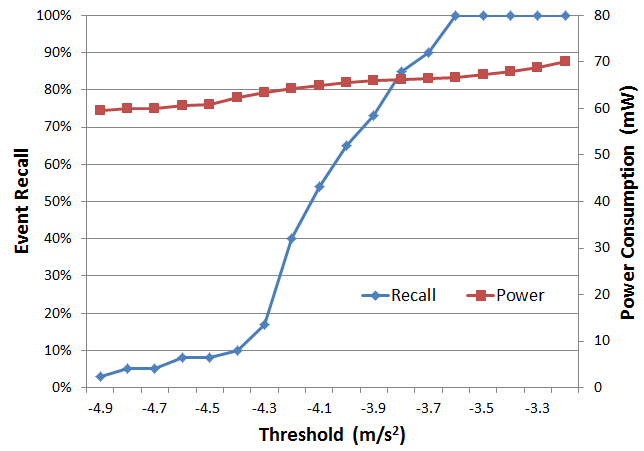
\includegraphics[width=3.1in]{wuc_hb_fft_group3.png}
	\caption{Threshold sensitivity for Headbutts.}
    \label{fig:wucHeadbuttFFTRecallPowerGroup3}
\end{figure}




\subsection{Human Traces}

Table~\ref{table:macrobenchmarks} shows the results from running the
step detector application on traces collected from three human
subjects.  Since these traces are not annotated with ground truth, we
use the steps detected by the Always Awake as the baseline for
determining recall.

Remarkably the results from these experiments show very similar
benefits to the synthetic experiments for runs with low and medium
levels of activity.  For example, the Smartsensor approach achieves
at least 91\% of the available power saving in each of the traces.

\begin{table*}[t]
\centering
{\small
    \begin{tabular}{|l|c|c|c|c|c|c|}
    \hline
	\multirow{2}{*}{Approach}		& \multirow{2}{*}{\parbox{2.2cm}{Sleep Interval (seconds)}}
												& \multicolumn{3}{c|}{\parbox{5.2cm}{Average Power (mW)}}
																								& \multirow{2}{*}{\parbox{1.5cm}{Average Recall}} \\ \cline{3-5}
									&			& Trace 1		& Trace 2		& Trace 3 		& 							\\ 
									&			& 37\% walking	& 22\% walking		& 20\% walking		& \\ \hline
	Always Awake					& 			& \multicolumn{3}{c|}{323} 						& 100\% \\ \hline
	\multirow{5}{*}{Duty Cycling}	& 2			& 329			& 330			& 330			& 97\%	\\ \cline{2-6}
									& 5			& 272			& 260			& 261			& 92\%	\\ \cline{2-6}
									& 10		& 220			& 195			& 198			& 82\%	\\ \cline{2-6}
									& 20		& 172			& 131			& 134			& 66\%	\\ \cline{2-6}
									& 30		& 148			& 104			& 106			& 57\%	\\ \hline
	\multirow{5}{*}{Batching}		& 2			& \multicolumn{3}{c|}{350} 						& 100\% \\ \cline{2-6}
									& 5			& \multicolumn{3}{c|}{186} 						& 100\% \\ \cline{2-6}
	 								& 10		& \multicolumn{3}{c|}{115} 						& 100\% \\ \cline{2-6}
	 								& 20		& \multicolumn{3}{c|}{80.1} 					& 100\% \\ \cline{2-6}
	 								& 30		& \multicolumn{3}{c|}{68.3} 					& 100\% \\ \hline
	Smartsensor				&			& 136			& 77.9			& 72.6			& 100\% \\ \hline
	Oracle				&			& 117.8			& 65.8			& 62.3			& 100\% \\ \hline



    \end{tabular}
}
	\caption{Event recall and average power for human traces.}
	\label{table:macrobenchmarks}
\end{table*}

%\subsection{Discussion}

%{\em TODO An integrated implemetation is likely to be more power
%  efficient. How does this affect these results?}
